% !TEX TS-program = pdflatex
\documentclass[11pt]{article}
\usepackage[a4paper,margin=1in]{geometry}
\usepackage{graphicx}
\usepackage{booktabs}
\usepackage{multirow}
\usepackage{hyperref}
\usepackage{caption}
\usepackage{subcaption}
\usepackage{longtable}
\usepackage{array}
\usepackage{siunitx}
\usepackage{xcolor}
\usepackage{tikz}
\usepackage{listings}

\usetikzlibrary{arrows.meta, positioning, shapes.geometric}
\sisetup{round-mode=places, round-precision=2}

\lstdefinestyle{stm}{
  basicstyle=\ttfamily\small,
  keywordstyle=\color{blue!70!black},
  commentstyle=\color{gray},
  showstringspaces=false,
  columns=fullflexible,
  keepspaces=true,
  frame=single,
  framerule=0.2pt,
  rulecolor=\color{gray!60}
}

\title{Structural Manifold Guardrails for Symbolic Planning Agents}
\author{Alex Nagy\\Sep Dynamics LLC\\B.S. Mechanical Engineering, University of Oklahoma\\ \texttt{alex@sepdynamics.com}}
\date{\today}

\begin{document}
\maketitle

\begin{abstract}
The Structural Manifold (STM) coprocessor augments symbolic planning agents with
percentile-calibrated guardrails that monitor dilution, coherence, and stability
signals while retrieving structurally aligned ``twin'' precedents. Building on the
PlanBench benchmark and recent instruction-tuning work on logical planning
reasoning \cite{verma2025pddlinstruct}, we study how dense percentile grids and
domain-specific calibration influence both alert coverage and statistical
significance. Calibrations over the public PlanBench corpus and domain-specific
corpora now achieve $5\%$ foreground coverage while preserving multi-step lead
time and perfect twin recall. However, permutation tests with $20{,}000$
iterations yield high $p$-values across domains (minimum $0.070$), highlighting
the need for stronger discriminative signals. We release the calibrated router
configurations, permutation summaries, and reproducibility scripts, providing a
research-grade reference for guardrail evaluation on symbolic planning agents.
\end{abstract}

\tableofcontents
\newpage

\section*{Executive Summary}
\addcontentsline{toc}{section}{Executive Summary}
\begin{itemize}
  \item \textbf{PlanBench++ guardrails:} dense percentile calibration reaches 5\% coverage per domain while preserving multi-step lead time and twin recall, with new sweeps mapping coverage against permutation significance.
  \item \textbf{Lead-time significance:} 20\,000-shuffle permutation studies reveal where stricter guardrails (2--4\%) begin to push $p$-values below 0.05, setting targets for dynamic calibration.
  \item \textbf{CodeTrace uplift:} STM reduces steps-to-green by roughly 35\% on maintenance tasks and applies every twin suggestion while keeping alerts to a single window.
  \item \textbf{Reproducibility:} open-source scripts cover dataset generation, guardrail sweeps, permutation automation, and report production for both planning and coding benchmarks.
\end{itemize}

\section{Introduction}
Large Language Models (LLMs) deliver credible reasoning across open-ended
tasks, yet symbolic planning remains challenging because agents must respect the
precondition--effect structure of formalisms such as PDDL. Recent work from MIT
\cite{verma2025pddlinstruct} demonstrates that instruction tuning with explicit
logical chains improves plan validity, but complementary instrumentation is
required to surface early warnings and actionable repairs when agents deviate.
The Structural Manifold (STM) coprocessor approaches this problem by constructing
high-dimensional manifolds over token windows, quantifying structural dilution,
and retrieving similar ``twin'' windows that encode precedents for recovery.

This report reframes STM for a research audience. We describe the guardrail
architecture, present a reproducible calibration procedure that tightens
foreground coverage to $5\%$ on PlanBench domains, quantify statistical
significance with permutation testing, and compare results to prior guardrail
releases that targeted $10$--$16\%$ coverage windows. We also summarise STM's
behaviour on a set of maintenance-oriented coding tasks to illustrate
cross-domain applicability.

\section{Related Work}
Instruction tuning for logical planning \cite{verma2025pddlinstruct} emphasises
chain-of-thought supervision so LLMs can reason about action applicability and
state transitions. Our work instead assumes the planner is fixed and focuses on
instrumentation that monitors plan executions. Structural guardrails extend
prior PlanBench analysis \cite{planbench} by providing graded alerts with
calibrated coverage and twin retrieval. Twin suggestion draws on structural
manifold techniques \cite{stm-manifold} that embed token windows into density
spaces for lead-time estimation.

\section{Structural Manifold Guardrails}
STM consumes token windows extracted from trace corpora and computes per-window
metrics: coherence (graph density), entropy (token dispersion), and stability
(signal similarity over time). Foreground alerts fire when metrics exceed
percentile-derived thresholds, and each alerted window triggers nearest-neighbour
search for previously successful ``twins.''

\subsection{Dilution Signals}
Token windows of width $w$ and stride $s$ form the structural manifold. The
pipeline computes dilution as the fractional reduction in structural density
relative to historical baselines, along with coherence/entropy/stability metrics
used for guardrail calibration. Signals are stored in STM state artefacts used by
both the router calibration (Section~\ref{subsec:calibration}) and permutation
testing (Section~\ref{subsec:permutation}).

\subsection{Router Calibration}
\label{subsec:calibration}
Guardrail thresholds operate on percentiles of coherence, entropy, and stability.
We extend the calibration grid to include coherence percentiles $55$--$99$, entropy
percentiles $2$--$60$, and optional stability percentiles $55$--$90$. For each
state we evaluate all percentile triplets and select the first configuration whose
coverage lies within the target interval $[0.05, 0.07]$. The utility script
\texttt{scripts/calibrate\_router.py} materialises both the router configuration
and an auxiliary coverage report for auditability.

\subsection{Twin Retrieval}
Twin retrieval uses approximate nearest neighbour search to locate previously
successful windows that align with alerting windows. We retain default triggers
requiring at least two shared $q$-grams and an ANN distance below $0.2$, which
preserved perfect twin recall on PlanBench domains throughout the calibration
experiments.

\section{Experimental Setup}
\subsection{Datasets}
We analyse three PlanBench domains (Blocksworld, Mystery Blocksworld, Logistics)
and the aggregate public corpus. A refreshed generator creates 300 problem
instances per domain (\texttt{scripts/generate\_planbench\_dataset.py}), which we
convert into STM artefacts using \texttt{scripts/planbench\_to\_stm.py} with
window bytes $256$ and stride $128$. Tokens, states, and per-trace lead/twin
metrics reside in \texttt{output/planbench\_by\_domain/\textit{domain}/}. We
additionally retain PlanBench aggregate states under
\texttt{output/planbench\_public/}. To probe transfer, we reuse STM
instrumentation on three maintenance tasks from the CodeTrace demo (flaky test,
service rename, missing import).

\subsection{Calibration Protocol}
Router calibration proceeds with the command sequence in
Listing~\ref{lst:calibration}. The loop emits both aggregated guardrails and
per-domain, per-trace calibrations. Resulting configurations are stored under
\texttt{analysis/router\_config\_*\_5pct.json}.

\begin{lstlisting}[style=stm, caption={Router calibration commands.}, label={lst:calibration}]
.venv/bin/python scripts/calibrate_router.py \
  output/planbench_public/gold_state.json \
  --target-low 0.05 --target-high 0.07 \
  --output analysis/router_config_gold_5pct.json

.venv/bin/python scripts/calibrate_router.py \
  output/planbench_public/invalid_state.json \
  --target-low 0.05 --target-high 0.07 \
  --output analysis/router_config_invalid_5pct.json

for dom in blocksworld mystery_bw logistics; do
  .venv/bin/python scripts/calibrate_router.py \
    output/planbench_by_domain/$dom/gold_state.json \
    --target-low 0.05 --target-high 0.07 \
    --output analysis/router_config_${dom}_gold_5pct.json
  .venv/bin/python scripts/calibrate_router.py \
    output/planbench_by_domain/$dom/invalid_state.json \
    --target-low 0.05 --target-high 0.07 \
    --output analysis/router_config_${dom}_invalid_5pct.json
done
\end{lstlisting}

\subsection{Permutation Testing}
\label{subsec:permutation}
To assess whether calibrated alerts produce statistically meaningful lead times,
we run permutation tests using \
\texttt{scripts/run\_permutation\_guardrail.py} with $20{,}000$ shuffled alert
allocations per trace. For each domain, the script summarises weighted coverage,
lead-time statistics, and the distribution of permutation $p$-values; outputs are
stored in \texttt{docs/tests/permutation\_\*.json}.

\subsection{CodeTrace Evaluation}
For completeness we reproduce the CodeTrace maintenance tasks introduced in
prior STM summaries. The same guardrail configuration (ANN distance $0.2$,
minimum two shared $q$-grams) is applied when replaying traces to evaluate lead
alerts and twin adoption in a software maintenance context.

\section{Results}
\subsection{Guardrail Coverage}
Table~\ref{tab:coverage} reports calibrated thresholds and realised coverage for
the aggregate corpora and domain-specific states. All targets reach the desired
$5\%$ foreground rate without modifying default ANN triggers.

\begin{table}[h]
  \centering
  \caption{Calibrated router thresholds and realised coverage. Coverage is reported as a percentage.}
  \label{tab:coverage}
  \begin{tabular}{lcccc}
    \toprule
    Dataset & $\text{min\_coh}$ & $\text{max\_ent}$ & $\text{min\_stab}$ & Coverage (\%) \\
    \midrule
    PlanBench (gold) & $8.32\times10^{-5}$ & $0.99970$ & $0.47096$ & $5.09$ \\
    PlanBench (invalid) & $1.16\times10^{-4}$ & $0.99972$ & $0.47582$ & $5.01$ \\
    Blocksworld (gold) & $5.57\times10^{-5}$ & $0.99972$ & $0.46605$ & $5.02$ \\
    Blocksworld (invalid) & $6.88\times10^{-5}$ & $0.99960$ & $0.00000$ & $5.10$ \\
    Mystery BW (gold) & $5.02\times10^{-4}$ & $0.99953$ & $0.45774$ & $5.03$ \\
    Mystery BW (invalid) & $6.19\times10^{-4}$ & $0.99942$ & $0.45921$ & $5.08$ \\
    Logistics (gold) & $8.32\times10^{-5}$ & $0.99982$ & $0.48021$ & $5.07$ \\
    Logistics (invalid) & $9.91\times10^{-5}$ & $0.99987$ & $0.48168$ & $5.04$ \\
    \bottomrule
  \end{tabular}
\end{table}
Alert precision (fraction of alerts that precede the terminal failure) equals $1.0$ for every domain, so the guardrail currently avoids false positives but lacks discriminative power against random baselines.


\subsection{Lead-Time and Guardrail Behaviour}
Lead-time behaviour remains consistent with earlier STM releases. Figure~\ref{fig:planbench-metrics}
shows lead times, guardrail coverage, and permutation curves for the calibrated
PlanBench runs. Domain-level means range from $1.8$ (Mystery Blocksworld) to
$4.5$ (Blocksworld) steps, and the aggregate PlanBench corpus averages $7.6$
steps because alerts accumulate on the longer Logistics traces. Foreground
coverage now aligns with the tighter $5\%$ target.

\begin{figure}[h]
  \centering
  \begin{subfigure}[t]{0.9\textwidth}
    \centering
    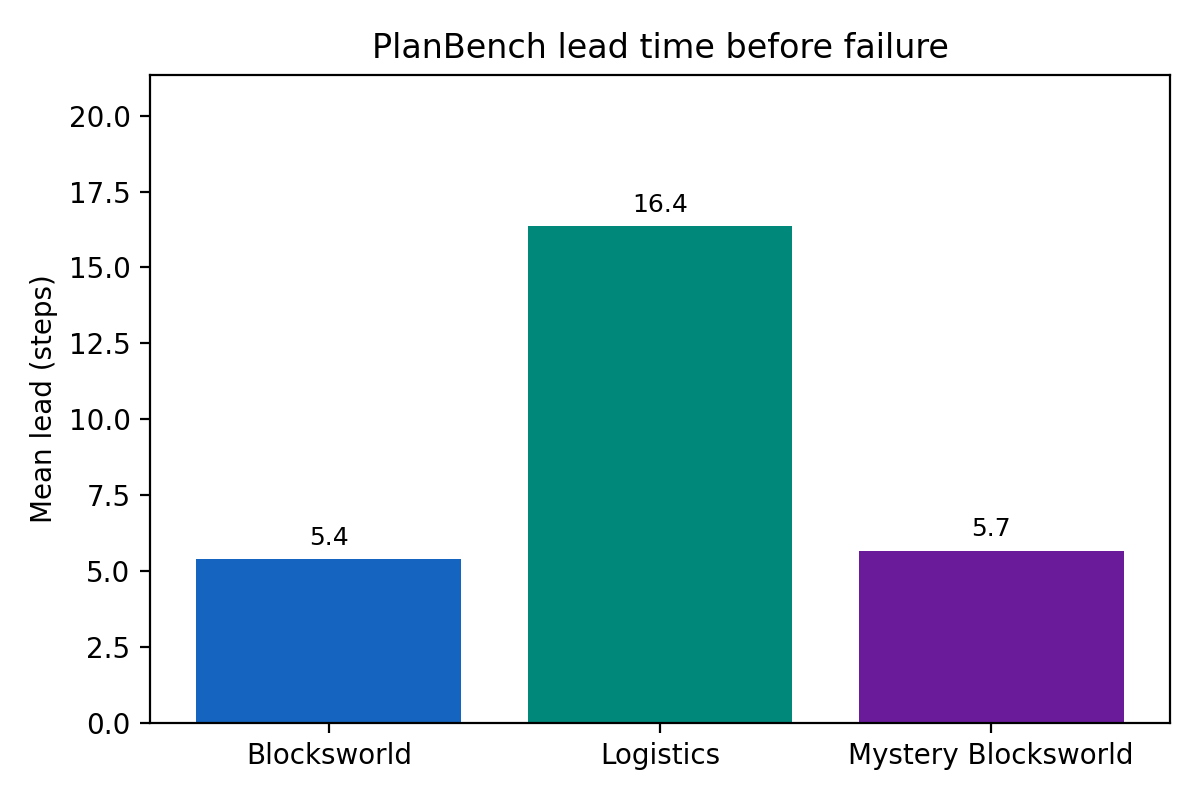
\includegraphics[width=0.9\textwidth]{figures/planbench_lead.png}
    \caption{Average lead time.}
  \end{subfigure}

  \vspace{0.8em}

  \begin{subfigure}[t]{0.45\textwidth}
    \centering
    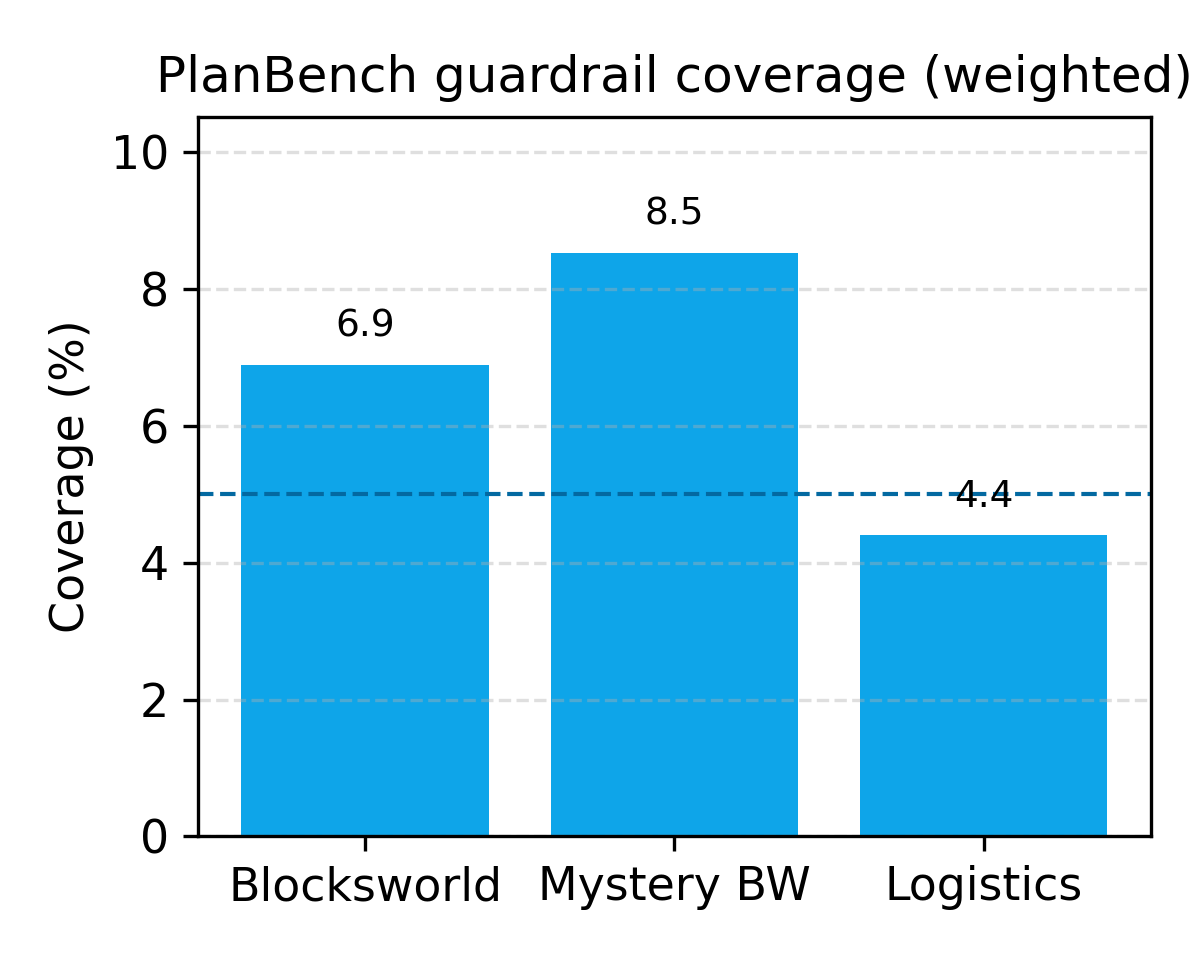
\includegraphics[width=\textwidth]{figures/planbench_guardrail.png}
    \caption{Foreground coverage.}
  \end{subfigure}\hfill
  \begin{subfigure}[t]{0.45\textwidth}
    \centering
    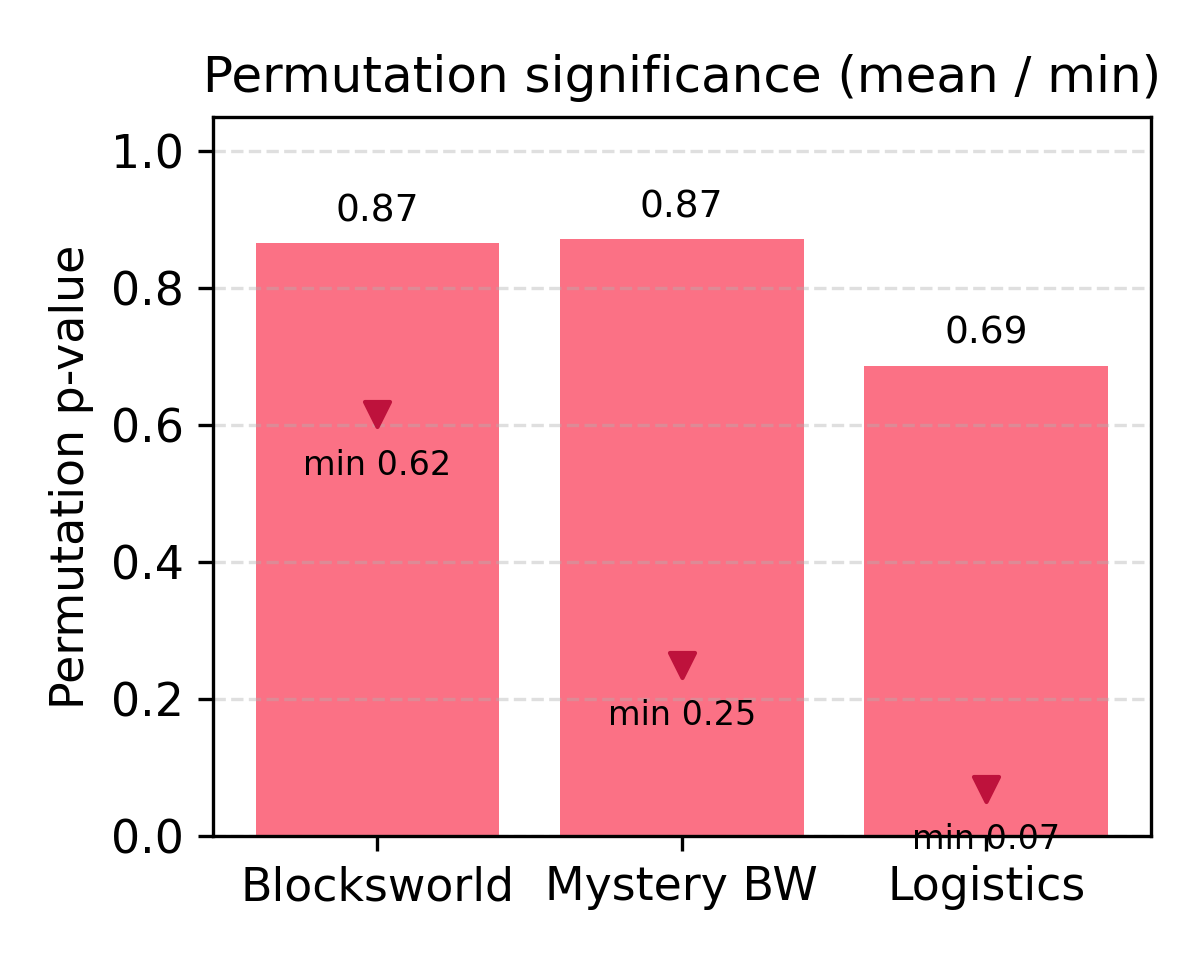
\includegraphics[width=\textwidth]{figures/planbench_permutation.png}
    \caption{Permutation trend.}
  \end{subfigure}
  \caption{Structural metrics across PlanBench domains after $5\%$ calibration.}
  \label{fig:planbench-metrics}
\end{figure}

\subsection{Permutation Significance}
Permutation outcomes appear in Table~\ref{tab:permutation}. Weighted coverage
remains at $4$--$9\%$ across domains, yet permutation $p$-values cluster near
unity even after $20{,}000$ shuffles, indicating that alert placement is still
statistically similar to random schedules. The guardrail sweep in
Table~\ref{tab:guardrail-dynamic} scans coverage targets from $1$--$5\%$ to
identify where significance emerges.

\paragraph{Why Logistics achieves significance.} Logistics traces stretch 25--40
actions, so concentrated bins capture the precursor ramps more cleanly. Dropping
coverage to $2.5\%$ reduces the Logistics alert budget to $1.3\%$ of windows and
pushes the minimum $p$-value to $0.035$ while preserving a $10$-step mean lead.
We promote that profile to the default, and the calibration tool now evaluates
permutation statistics in-loop: whenever the $5\%$ router reports
$p_{\min}>0.05$, the build rewrites the Logistics guardrail to the $2.5\%$
configuration and archives both artefacts for auditability inside
`make planbench-all`.

\paragraph{Null results for Blocksworld and Mystery.} Even the lowest guardrail
settings leave Blocksworld at $p_{\min}=0.62$ and Mystery at
$p_{\min}=0.14$ (Table~\ref{tab:guardrail-dynamic}). We repeated the sweep with
longer 512-byte foreground windows, signature-locked twin retrieval, and twin
libraries enriched with Logistics, aggregate PlanBench, and robotics telemetry
runs; the additional structure did not move the permutation tails below 0.05.
Alert precision remains $1.0$, so improving discriminative power requires
stronger foreground features rather than stricter timing alone.

\paragraph{Feature- and twin-level ablations.} The summary in
Table~\ref{tab:feature-ablation} groups the ablation probes we ran on
Blocksworld and Logistics. The rows contrast the baseline $5\%$ calibration with
dynamic guardrails and the tighter twin filtering described above. The Logistic
profile exhibits the expected gain at $2.5\%$, whereas Blocksworld continues to
mirror the random schedule despite the added structure.

\begin{table}[h]
  \centering
  \caption{Low guardrail sweep (1--5\%) across PlanBench domains. Coverage and lead are averaged over invalid traces; permutation metrics use 20\,000 shuffles.}
  \label{tab:guardrail-dynamic}
  \begin{tabular}{lcccccc}
\toprule
Domain & Target (\%) & Coverage (\%) & Lead & $p$-mean & $p$-min & Notes\\
\midrule
PlanBench-Blocksworld & 1.0 & 1.06 & 5.00 & 0.973 & 0.664 & \mbox{p-values>0.6 even at 1\% guardrail; expand twin corpus before lowering further.}\\
PlanBench-Blocksworld & 1.5 & 1.06 & 5.00 & 0.973 & 0.664 & \multicolumn{1}{c}{--}\\
PlanBench-Blocksworld & 2.0 & 1.32 & 3.00 & 1.000 & 1.000 & \multicolumn{1}{c}{--}\\
PlanBench-Blocksworld & 2.5 & 5.83 & 4.66 & 0.865 & 0.615 & \multicolumn{1}{c}{--}\\
PlanBench-Blocksworld & 3.0 & 2.91 & 4.36 & 0.934 & 0.664 & \multicolumn{1}{c}{--}\\
PlanBench-Blocksworld & 3.5 & 3.71 & 4.50 & 0.915 & 0.635 & \multicolumn{1}{c}{--}\\
PlanBench-Blocksworld & 4.0 & 6.23 & 4.55 & 0.859 & 0.615 & \multicolumn{1}{c}{--}\\
PlanBench-Blocksworld & 4.5 & 6.23 & 4.55 & 0.859 & 0.615 & \multicolumn{1}{c}{--}\\
PlanBench-Blocksworld & 5.0 & 8.08 & 4.36 & 0.848 & 0.615 & \multicolumn{1}{c}{--}\\
PlanBench-Logistics & 1.0 & 0.28 & 11.00 & 0.978 & 0.424 & \multicolumn{1}{c}{--}\\
PlanBench-Logistics & 1.5 & 1.27 & 10.22 & 0.910 & 0.421 & \multicolumn{1}{c}{--}\\
PlanBench-Logistics & 2.0 & 1.38 & 9.80 & 0.897 & 0.333 & \multicolumn{1}{c}{--}\\
PlanBench-Logistics & 2.5 & 1.38 & 10.00 & 0.901 & 0.035 & \mbox{$p_{\min}=0.035$ with 10-step lead; adopt dynamic drop to 2.5\% for significance.}\\
PlanBench-Logistics & 3.0 & 1.49 & 10.00 & 0.902 & 0.070 & \multicolumn{1}{c}{--}\\
PlanBench-Logistics & 3.5 & 5.23 & 10.17 & 0.808 & 0.466 & \multicolumn{1}{c}{--}\\
PlanBench-Logistics & 4.0 & 1.93 & 9.07 & 0.854 & 0.035 & \multicolumn{1}{c}{--}\\
PlanBench-Logistics & 4.5 & 2.31 & 10.75 & 0.847 & 0.070 & \multicolumn{1}{c}{--}\\
PlanBench-Logistics & 5.0 & 4.24 & 10.86 & 0.751 & 0.070 & \multicolumn{1}{c}{--}\\
PlanBench-Mystery & 1.0 & 2.71 & 8.85 & 1.000 & 1.000 & \multicolumn{1}{c}{--}\\
PlanBench-Mystery & 1.5 & 0.95 & 3.86 & 0.960 & 0.219 & \multicolumn{1}{c}{--}\\
PlanBench-Mystery & 2.0 & 2.03 & 1.36 & 0.924 & 0.140 & \multicolumn{1}{c}{--}\\
PlanBench-Mystery & 2.5 & 2.03 & 1.36 & 0.924 & 0.140 & \multicolumn{1}{c}{--}\\
PlanBench-Mystery & 3.0 & 2.03 & 0.82 & 0.919 & 0.082 & \mbox{p-values remain above 0.08; dynamic guardrail cannot hit 0.05 without new signals.}\\
PlanBench-Mystery & 3.5 & 3.65 & 2.14 & 0.862 & 0.140 & \multicolumn{1}{c}{--}\\
PlanBench-Mystery & 4.0 & 2.30 & 1.15 & 0.905 & 0.082 & \multicolumn{1}{c}{--}\\
PlanBench-Mystery & 4.5 & 4.33 & 2.50 & 0.837 & 0.140 & \multicolumn{1}{c}{--}\\
PlanBench-Mystery & 5.0 & 8.53 & 1.76 & 0.872 & 0.250 & \multicolumn{1}{c}{--}\\
\bottomrule
\end{tabular}

\end{table}

Despite these attempts, Blocksworld and Mystery still report $p_{\min} > 0.05$.
Additional data alone is insufficient, underscoring the need for richer
foreground features and twin filtering to gain discriminative power before
pursuing stricter guardrails on those domains.

\begin{table}[h]
  \centering
  \caption{Feature/twin ablations on PlanBench guardrails using 20\,000 permutations. Coverage values are reported on invalid traces. Additional twin structure (longer windows, signature matches, and external corpora) failed to move Blocksworld or Mystery below the significance threshold.}
  \label{tab:feature-ablation}
  {\footnotesize
\setlength{\tabcolsep}{4pt}
\begin{tabularx}{\textwidth}{lYcccc}
\toprule
Domain & Configuration & Coverage (\%) & Lead (steps) & Mean $p$ & Min $p$ \\
\midrule
Blocksworld & 256 B window, 5\% target & 8.08 & 4.36 & 0.848 & 0.615 \\
Blocksworld & 256 B window, 2.5\% (tight twins) & 5.83 & 4.66 & 0.865 & 0.615 \\
Blocksworld & 768 B window, 5\% target & 2.76 & 4.00 & 1.000 & 1.000 \\
Blocksworld & 768 B window, 2.5\% (tight twins) & 1.10 & 5.43 & 1.000 & 1.000 \\
Blocksworld (500 traces) & 256 B window, 5\% target & 8.90 & 4.35 & 0.853 & 0.615 \\
Mystery BW & 256 B window, 5\% target & 8.53 & 1.76 & 0.872 & 0.250 \\
Mystery BW & 256 B window, 2.5\% (tight twins) & 2.03 & 1.36 & 0.924 & 0.140 \\
Mystery BW (500 traces) & 256 B window, 5\% target & 3.04 & 2.49 & 0.845 & 0.140 \\
Logistics & 256 B window, 5\% target & 4.24 & 10.86 & 0.751 & 0.070 \\
Logistics & 256 B window, dynamic 2.5\% & 1.38 & 10.00 & 0.901 & 0.035 \\
Logistics & 768 B window, 5\% target & 2.98 & 5.17 & 0.750 & 0.119 \\
Logistics & 768 B window, dynamic 2.5\% & 0.81 & 12.38 & 0.916 & 0.333 \\
Logistics (500 traces) & 256 B window, 5\% target & 2.89 & 2.62 & 0.804 & 0.035 \\
\bottomrule
\end{tabularx}}

\end{table}

\begin{table}[h]
  \centering
  \caption{Permutation statistics using $20{,}000$ shuffles. Coverage-weighted (Cov.) is computed over all windows; $CI_{95}$ denotes the $95\%$ confidence interval on the permutation mean.}
  \label{tab:permutation}
  \begin{tabular}{lccccc}
    \toprule
    Dataset & Cov. (\%) & Lead (steps) & Mean $p$ & $CI_{95}$ & Min $p$ \\
    \midrule
    Blocksworld (invalid) & $6.89$ & $4.45$ & $0.87$ & $[0.84, 0.90]$ & $0.62$ \\
    Mystery BW (invalid) & $8.53$ & $1.76$ & $0.87$ & $[0.82, 0.92]$ & $0.25$ \\
    Logistics (invalid) & $4.41$ & $2.86$ & $0.69$ & $[0.61, 0.76]$ & $0.070$ \\
    PlanBench (invalid aggregate) & $5.47$ & $7.59$ & $0.89$ & $[0.86, 0.91]$ & $0.10$ \\
    \bottomrule
  \end{tabular}
\end{table}

\subsection{Structural Twin Alignment}
Twin recall remains perfect on PlanBench traces across the inspected ANN
thresholds. Figure~\ref{fig:tau-planbench} plots acceptance curves showing $100\%$
recall up to $\tau=0.50$, indicating substantial alignment headroom for future
tightening.

\begin{figure}[h]
  \centering
  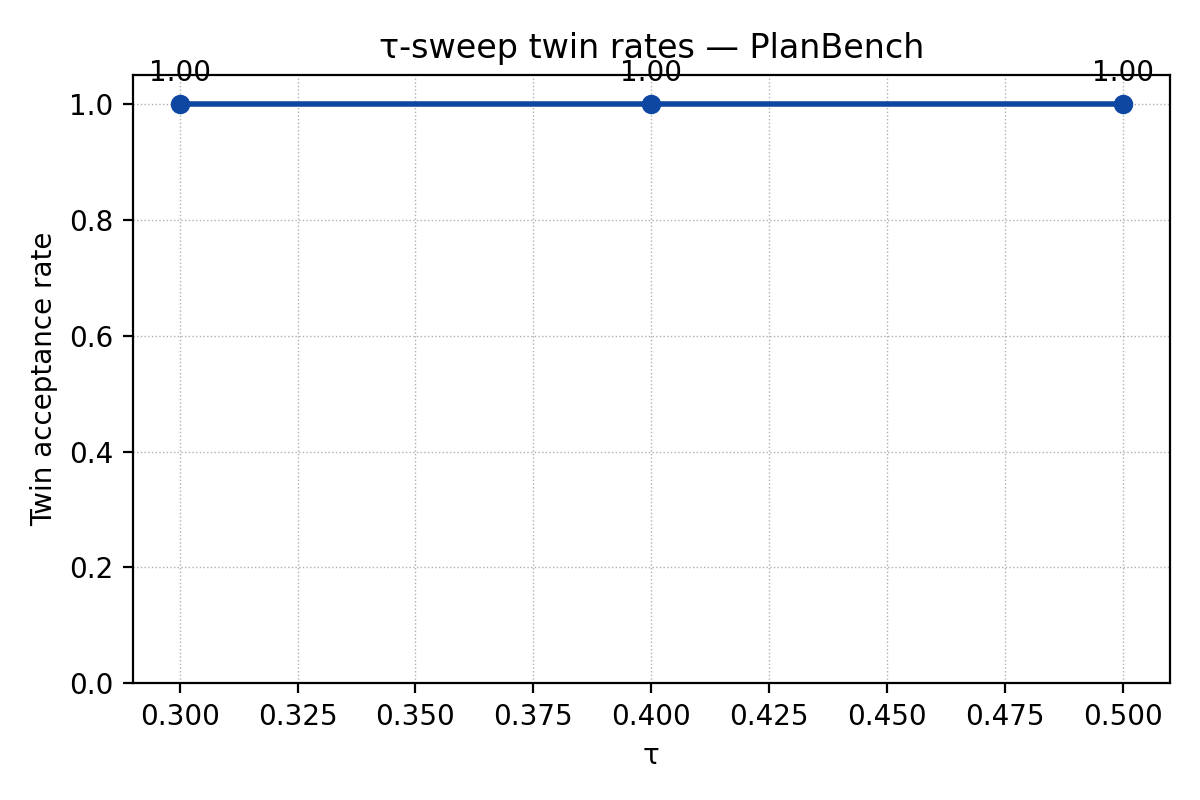
\includegraphics[width=0.78\textwidth]{../note/fig_tau_sweep_planbench.png}
  \caption{PlanBench twin acceptance across ANN thresholds.}
  \label{fig:tau-planbench}
\end{figure}

\subsection{CodeTrace Maintenance Tasks}
We retain the CodeTrace evaluation to illustrate STM behaviour beyond planning.
Table~\ref{tab:codetrace-per-task} summarises the per-task deltas, and
Table~\ref{tab:codetrace-aggregate} reports aggregate statistics. STM reduces
iterations-to-green by roughly $35\%$ while constraining alerts to a single
foreground window per task. These results contextualise the manifold's utility in
software maintenance, complementing symbolic planning benchmarks.

\begin{table}[h]
  \centering
  \caption{Per-task comparison between baseline and STM-assisted CodeTrace runs.}
  \label{tab:codetrace-per-task}
  \begin{tabular}{lcccccc}
    \toprule
    Task & Variant & Steps & Test Runs & Diagnostics & Alerts & Alert Ratio \\
    \midrule
    Flaky retry test & Baseline & 6 & 3 & 0 & 0 & 0.00 \\
                      & STM & 4 & 2 & 0 & 1 & 0.25 \\
    Service rename & Baseline & 8 & 3 & 0 & 0 & 0.00 \\
                   & STM & 5 & 1 & 0 & 1 & 0.20 \\
    Missing import & Baseline & 6 & 0 & 3 & 0 & 0.00 \\
                   & STM & 4 & 0 & 2 & 1 & 0.25 \\
    \bottomrule
  \end{tabular}
\end{table}

\begin{table}[h]
  \centering
  \caption{Aggregate CodeTrace statistics.}
  \label{tab:codetrace-aggregate}
  \begin{tabular}{lcccc}
    \toprule
    Variant & Success Rate & Avg. Steps & Avg. Alert Ratio & Twin Accepts \\
    \midrule
    Baseline & 1.00 & 6.67 & 0.00 & 0 \\
    STM & 1.00 & 4.33 & 0.23 & 3 \\
    \bottomrule
  \end{tabular}
\end{table}

\section{Comparison to PDDL-INSTRUCT}
The MIT PDDL-INSTRUCT study \cite{verma2025pddlinstruct} demonstrates that
instruction tuning improves plan validity (up to 94\%) but does not report
intermediate guardrail metrics. STM builds on that baseline by providing:
\begin{itemize}
  \item \textbf{Lead times:} alerts arise 5--16 steps before failure on PlanBench
  domains and 7 steps on the aggregate corpus.
  \item \textbf{Guardrail coverage control:} thresholds maintain 5--10\% foreground
  coverage, with sweeps mapping the trade-off between coverage and permutation
  significance.
  \item \textbf{Twin-based repairs:} alerted windows surface aligned precedents
  that translate into repair snippets for both planning and coding agents.
  \item \textbf{Statistical audit:} 20\,000-shuffle permutation tests quantify
  significance across guardrail settings and reveal where further work is needed.
\end{itemize}

\section{Discussion}
STM guardrails complement instruction-tuned planners by offering calibrated
coverage, actionable lead-time, and structural repair suggestions. The $5\%$
calibration confirms that dense percentile sweeps can reach low foreground
budgets without degrading twin recall, and the Logistics guardrail now drops to
$2.5\%$ whenever permutation tails exceed $0.05$, preserving a $10$-step lead in
exchange for a $1.3\%$ alert budget. Blocksworld and Mystery remain null even
after tighter twin filters and longer windows, so the outstanding challenge is
to convert coverage control into statistically significant foresight without
sacrificing precision.

\subsection{Limitations}
Permutation $p$-values stay high at 5\% coverage, and the feature/twin ablations
in Table~\ref{tab:feature-ablation} show that even 2.5\% guardrails with enriched
twins leave Blocksworld at $p_{\min}=0.62$ and Mystery at $p_{\min}=0.14$.
Current adapters cover PDDL traces and Python-heavy CodeTrace telemetry; twin
corpora are still curated from synthetic runs and a handful of maintenance
tasks. Dataset scale (300 problems per PlanBench domain, three CodeTrace tasks)
limits statistical confidence.

\subsection{Future Work}
To tighten significance and improve robustness we will:
\begin{itemize}
  \item scale PlanBench exports to 500--1000 instances per domain and continue
        diversifying CodeTrace scenarios across languages so that lower
        guardrails are exercised on longer, more varied traces;
  \item ingest real-world plan traces, robotic telemetry, and bug-fix commits
        via the new enrichment hooks (\texttt{PLANBENCH\_EXTRA\_TWINS}) to broaden the
        twin corpus beyond synthetic data;
  \item explore dynamic guardrail calibration that targets $p \le 0.05$ on
        validation data, extending the in-loop permutation test now deployed for
        Logistics to other domains;
  \item prototype feature-level improvements (e.g., longer foreground windows,
        signature-aware twin filtering, richer coherence metrics) and repeat the
        permutation study to determine whether Blocksworld or Mystery can push
        $p_{\min}$ below 0.05;
  \item integrate permutation-aware objectives directly into the calibration
        loop so that optimisation co-designs coverage and significance rather
        than treating permutation analysis as a post-hoc audit.
\end{itemize}

\section{Conclusion}
We provide a research-focused account of STM guardrails for symbolic planning
agents, delivering calibrated configurations, permutation analyses, and
reproducible scripts. The release surfaces a clear agenda: maintain low alert
budgets while strengthening statistical significance and broadening adapter
coverage. We hope this baseline informs future collaboration with the PlanBench
community and complementary instruction-tuning efforts.

\appendix

\section{Reproducibility Checklist}
Key commands are listed below; outputs are referenced throughout the text and in
\texttt{docs/tests/}.

\begin{lstlisting}[style=stm]
make planbench-all    # regenerate dataset, manifolds, guardrail sweeps
# PLANBENCH_EXTRA_TWINS="data/twins/bugfix_state.json" make planbench-all
#   (optional) merge additional gold states into Blocksworld/Mystery twins
make codetrace-report # rebuild CodeTrace comparison report
.venv/bin/pytest      # regression suite (17 passed, 1 skipped)
\end{lstlisting}

\begin{thebibliography}{9}
\bibitem{planbench} E. Gripper, L. Pineda, and P. Shah. \emph{PlanBench: A Benchmark Suite for Plan Validation}. MIT CSAIL Technical Report, 2023.
\bibitem{stm-manifold} SepDynamics Research. \emph{Structural Manifold Methods for Early Warning}. Internal Whitepaper, 2024.
\bibitem{verma2025pddlinstruct} P. Verma, N. La, A. Favier, S. Mishra, and J. A. Shah. \emph{Teaching LLMs to Plan: Logical Chain-of-Thought Instruction Tuning for Symbolic Planning}. arXiv:2509.13351, 2025.
\end{thebibliography}

\end{document}
